\section{CoCo Dataset}
In this section, we first present samples in our dataset. Next, we describe our data collection process, including text crawling, phrase pre-selecting, annotation, auto-generation and dataset validation. To better understand our CoCo dataset, we also conduct an analysis on the characteristics of all samples. General framework of dataset collection is shown in Figure \ref{fig:framework}.\JQ{和下边标题没有对应}

\begin{figure}
	\centering
	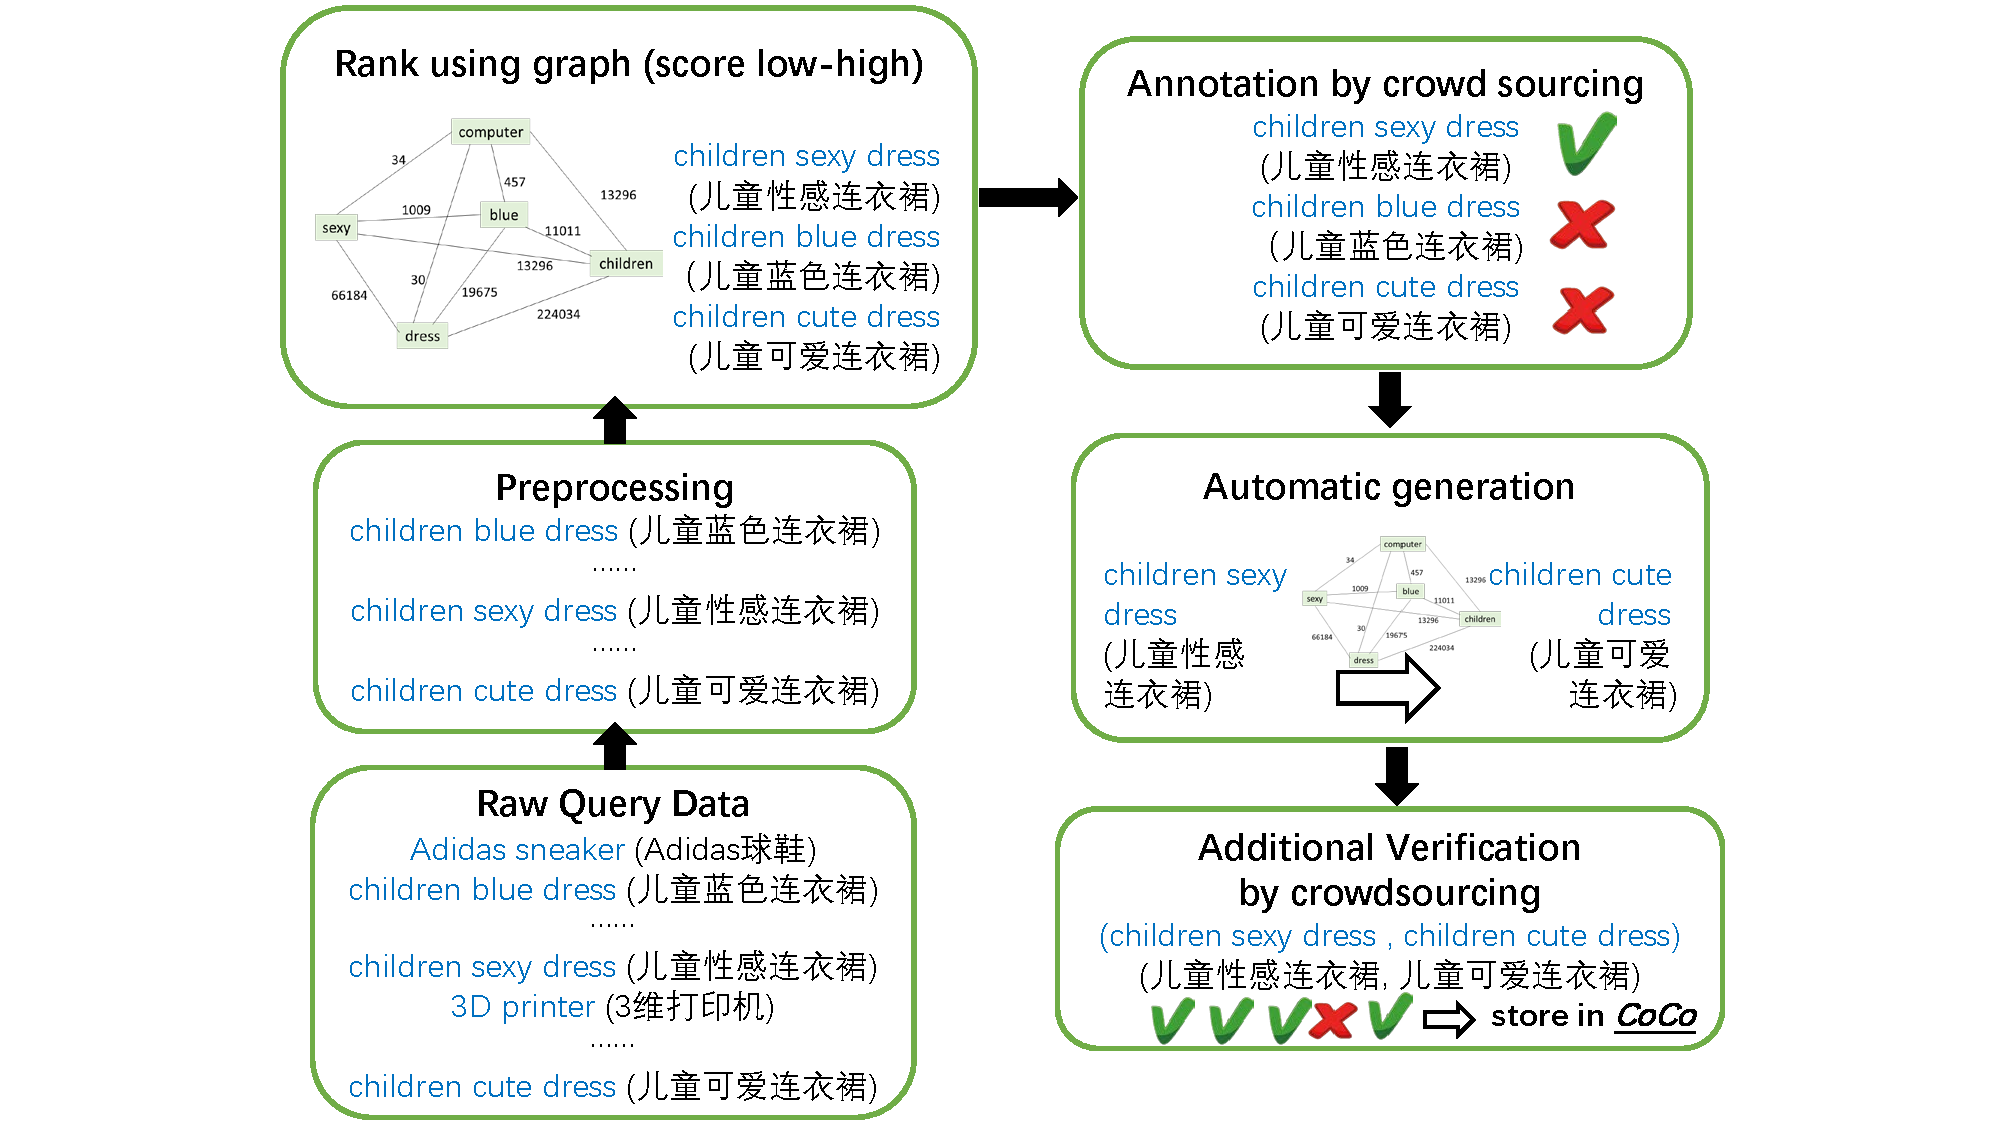
\includegraphics[width=\columnwidth]{images/framework.pdf}
	\caption{CoCo dataset collection process}
	\label{fig:framework}
\end{figure}

\subsection{Dataset Introduction}
Each instance in our CoCo dataset is %composed of 
%two short phrases and one label
a triple: $\{p_1, p_2, l\}$,
%Formally, each instance in our CoCo dataset is composed of 2 short phrases and 4 options: $\{p_1, p_2, r_1, r_2, r_3, r_4\}$. 
where $p_1$ and $p_2$ are two similar phrases focusing on the same subject
but with different modifiers.
However, only one of them is more plausible according to common sense. 
$l$ is the label which indicates the index of correct phrase. 
Therefore, the whole task can be seen as a binary classification problem 
and we use Accuracy as evaluation metric. 
%For the more unreasonable one, four options $\{r_1, r_2, r_3, r_4\}$ are offered to be chosen as the reason of being unreasonable. For both tasks, we use accuracy score to do the evaluation.
%\mx{Absence of dataset size}

\subsection{Raw Data Preprocessing}
%Alibaba inc offers us 
%We crawl %\mx{How to say??} 
We crawl search queries from a popular e-commerce platform 
where some noisy and meaningless queries are filtered
through query normalization including lexical error corrections and query rewriting.
We further filter out qeuries including numbers and English chars and remain  those queries that only composed of Chinese characters. 
After that, 4,081,254 common queries are left. 
These queries contain characters of length in range of 2 to 15, and 4.73 on average. The number of words\footnote{Word segmentations are done by using tools trained on E-commerce data in advance.} in queries is distributed between 2 to 8 and 2.07 on average.
%As for the number of words, queries distribute between 2 to 8, and 2.07 on average, 
The details of char and word number distribution is shown in Figure \ref{fig:wordDist}. 

\JQ{图得改:标题samples要留吗 0??保留几位小数?}
%\mx{figure or table is needed for words 2-8 or chars?}

\begin{figure}
	\centering
	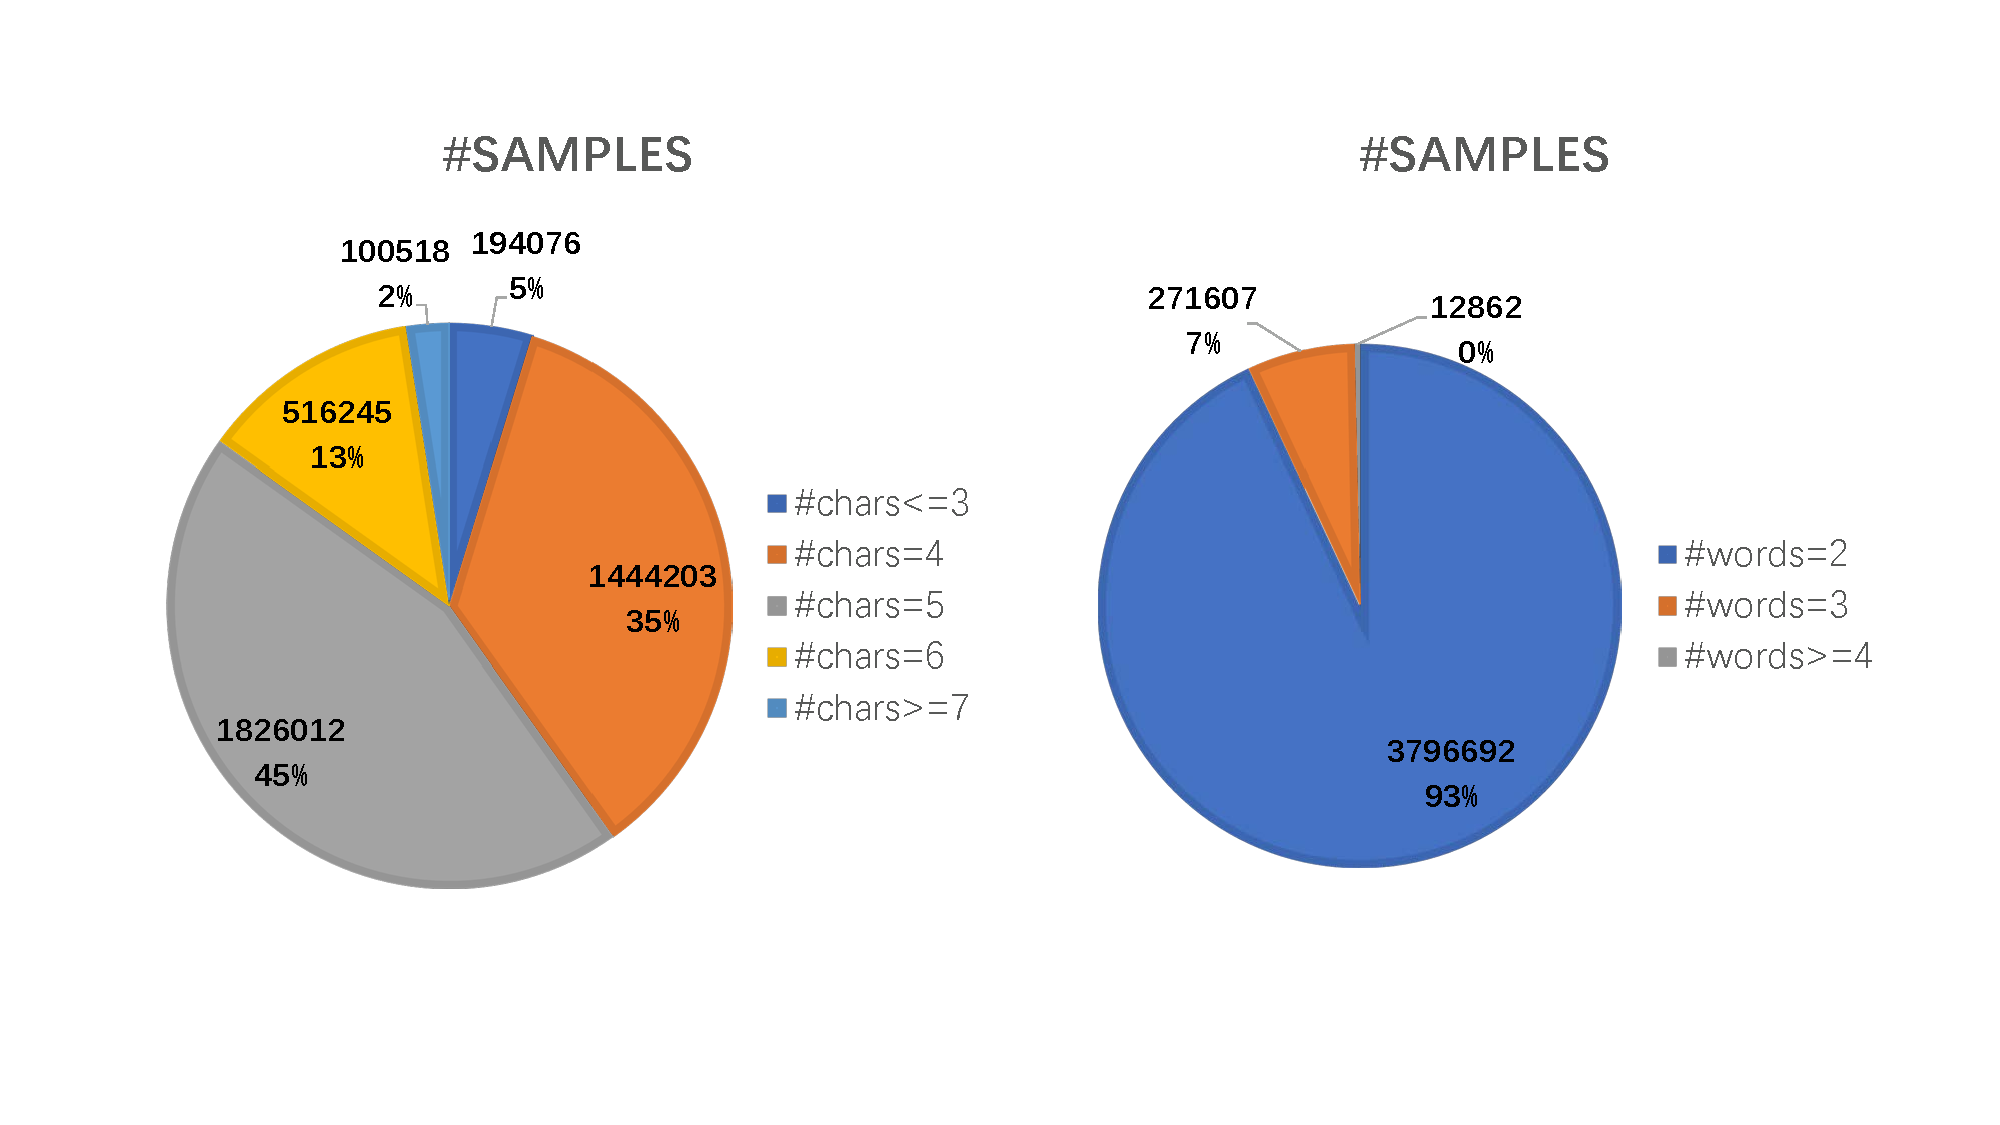
\includegraphics[width=0.95\columnwidth]{images/distributionWords.pdf}
	\caption{Char and word number distribution of raw data after preprocessing}
	\label{fig:wordDist}
\end{figure}

%\KZ{Words are too small in figure 1.}

%!!! Should give some statistics of this big table, ex. show length. 
%Besides, some modifications like query rewriting to make it clearer or lexical error corrections are also done. (query normalization) 


%\subsection{Preprocessed Data Overview}
\subsection{Auto-generation of CoCo pairs}
We define \textit{positive samples} as those phrases that have commonsense contradiction, and \textit{negative samples} as other phrases. 
%Our target is to get pairs of high-quality similar positive/negative samples as much as possible.
%Our target is to get positive samples as much as possible. 
%from the large query table.

To have a preliminary understanding over this whole table, we first randomly select 10,000 samples from preprocessed raw data and do the human annotation. 
%\mx{10000 need to be re-sampled, some samples that 1 word or have not-Chinese chars should be replaced.}
Among all selected samples, we find 292 positive samples and 9708 negative samples. It should be noticed that positive samples are much rarer than negative ones, only accounts for 2.92\%. Obviously, directly annotating the original collection of queries to get more negative\JQ{positive?} samples are not efficient.
%Therefore, we come up with two methods to get positive samples.
Therefore, we come up with two methods to get expected phrase pairs in CoCo dataset more efficiently: \textbf{Random generation} and \textbf{Filter using graph}. 

\subsubsection{Random Generation}
%As there are lots of negative samples, we consider to directly generate positive samples by randomly replacing 
%According to the statistics of preliminary human annotation, it is easier to get negative\JQ{positive} samples. %Hence, we consider 
The most nature and naive way is to directly generate associated similar positive samples starting with those negative annotated ones. %The following are our generation steps:
To check the effectiveness of this simple idea, we do the following experiments on a small dataset:
\begin{enumerate}
	\item Randomly select 100 high-quality negative samples, where \textit{high-quality} means:
	\begin{itemize}
		%\item [-] the query contains and only contains one subject, with one or several modifiers. For example, "skirt dress" is not satisfies because of two subjects; "cute dress" is a high-quality one.
		\item [-] \textit{stylistic} modifiers are clearly defined if exist, such as ``creative", ``personalized", ``popular" and etc.\JQ{有个stylistic modifiers字典之类的?}
		\item [-] modifiers in categories of \textit{nation} and \textit{color} should be paid more attention on. These two kinds of modifiers are versatile in most cases, for example, dress could be modified by all nations or colors, such as ``American dress", ``French dress", ``green dress" or ``red dress" and etc. However, some cases are special as they have intrinsic geographic characteristics (ex: ``Chinese dumplings") or color characteristics (ex: ``blue sea").\JQ{这个不是high-quality的标准吧?}
		\item [-] without brand name or people name. %(include actors).   
		\item [-] phrase is clear and the words used are common enough.	\JQ{common如何定义}
	\end{itemize}
	%\item To ensure that the candidate 100 negative samples are common and clear enough, we use official released "BERT-Base, Chinese" model \footnote{https://github.com/google-research/bert} to calculate perplexity of the choose 100 negative samples and replace those $PPL>=1000$ (9 among 100 for the first time) by other re-selected high-quality negative samples until all the selected negative samples satisfy $PPL<1000$. Here are the steps of calculating perplexity:
	%\begin{itemize}
	%	\item [-] As the vocabulary of original BERT Chinese model is on the level of characters, we just mask each character one by one for each query.
	%	\item [-] Fetch the probability of "MASK" being the associated character on the last layer, note as:\\$P(w_i) = P(w_i|w_1,...,w_{i-1},w_{i+1},...,w_n)$
	%	\item [-] For each query, we calculate perplexity as: \\
	%	$PPL(query) = e^{-(\sum_{i=1}^{n}logP_{i})/n}$  
	%\end{itemize}
	\item For each query, we randomly replace one of its word using vocabulary according to the following rules:
	\begin{itemize}
		\item [-] 
		%ensure consistency of word property itself, respecting the original Part-Of-Speech pattern. 
		ensure the consistency of the Part-Of-Speech pattern
		%which means subject replaced by subject, modifier replaced by modifier.
		\item [-] %ensure identity of word length, which means the replaced word should have the same length with the original word.
		ensure the identity of word length, because our further evaluation uses the perplexity (PPL) which is averaged by length during calculation. 
		%Notice that perplexity (PPL) is averaged by length during calculation, if one short modifier is replaced by a much longer modifier, even the new modifier does not match the subject, the new generated sample may get a lower ppl score as the new modifier itself is smooth and long enough to pull down the ppl score. Here is an example: "blue sky" vs "super cute green sky".
	\end{itemize} 
\end{enumerate}

Finally, ten positive samples are generated for each chosen negative sample, leading to 1000 pairs. We use one of the pretrained language model BERT to distinguish the more reasonable phrase from each pair. Perplexity (PPL) score is used as the evaluation metric: the pair with lower PPL will be considered as the more reasonable one.

Here are the steps of calculating PPL for a query $\{w_1 w_2 ... w_n\}$ by using the pretrained model BERT:
\begin{itemize}
	\item [-] As the vocabulary of original BERT Chinese model is trained on the level of characters, we just mask each character one by one for each query.
	\item [-] Fetch the probability of "MASK" being the associated character on the last layer\JQ{有点没看懂}, note as:\\$P(w_i) = P(w_i|w_1,...,w_{i-1},w_{i+1},...,w_n)$
	\item [-] For each query, we calculate perplexity as: \\
	$PPL(query) = e^{-(\sum_{i=1}^{n}logP_{i})/n}$  
\end{itemize}

There are totally 906 pairs that BERT judges correctly. The accuracy achieves 90.6\%. We also find that some pairs themselves can not be distinguished as both phrases are reasonable, such as ``Qing Dynasty teapo''(清朝茶碗) vs ``archaistic teabowl''(仿古茶碗). \JQ{这个pair怎么不符合generation呢}%The result shows that BERT really learns some useful statistical knowledge during pretraining stage.

However, after viewing all generated samples, %the randomly generated samples 
%they are indeed not high-quality 
they are indeed far away being a good dataset used for evaluating common sense, as there are some obviously strange combination such as ``cute shoe" vs ``bushy shoe", ``salty tofu" vs ``salty gypsum". \JQ{这个pair怎么不符合generation呢}
%this result also demonstrates that the randomly generated

Therefore, we decide to use another way to get pairs where phrases are more similar, more plausible, and with higher quality.

%\subsubsection{Further filter}
\subsubsection{Filter Using Graph}
%As statistics of human annotation show that there are only 2.92\% positive phrases if randomly sample from preprocessed raw data, directly annotation to get a large corpus of positive phrases are laborious. We aim at increasing the estimated proportion of positive samples and then applying human annotation to save time.

This method is based on the idea that \textit{popular query will have a larger probability to be reasonable}. We propose to construct a net of correlation weighted with co-occurrences between terms by using a large user queries corpus.

\textit{Step1: Positive samples preselecting}

%With the help of Alibaba inc, we obtain 
We first crawled user queries on e-commerce platform with data masking among 7 days (2019.07.15-2019.07.21). After filtering those queries that only have one word and keeping queries which are only formed by Chinese characters, we obtained 303,285,752 candidates in all. Then we analyze each query to get co-occurrence of each word pair, and gradually enrich the correlation net. 
For example, from the query ``sexy blue dress", we will get three word pairs (sexy, dress), (blue, dress) and (sexy, blue). Notice that the edge in our net does not have directions and the order of words is neglected.
% in word pairs is of no importance.
Besides, word synonyms are combined together using a Chinese synonym dictionary provided by HIT-SCIR\footnote{https://ltp-cloud.com/download/}.
After constructing net, the weight of each edge in the graph represents the frequency %number of times 
that this word pair was observed in the whole crawled user query corpus. A fragment of our constructed net is shown in Figure \ref{fig:net}.

\begin{figure}
	\centering
	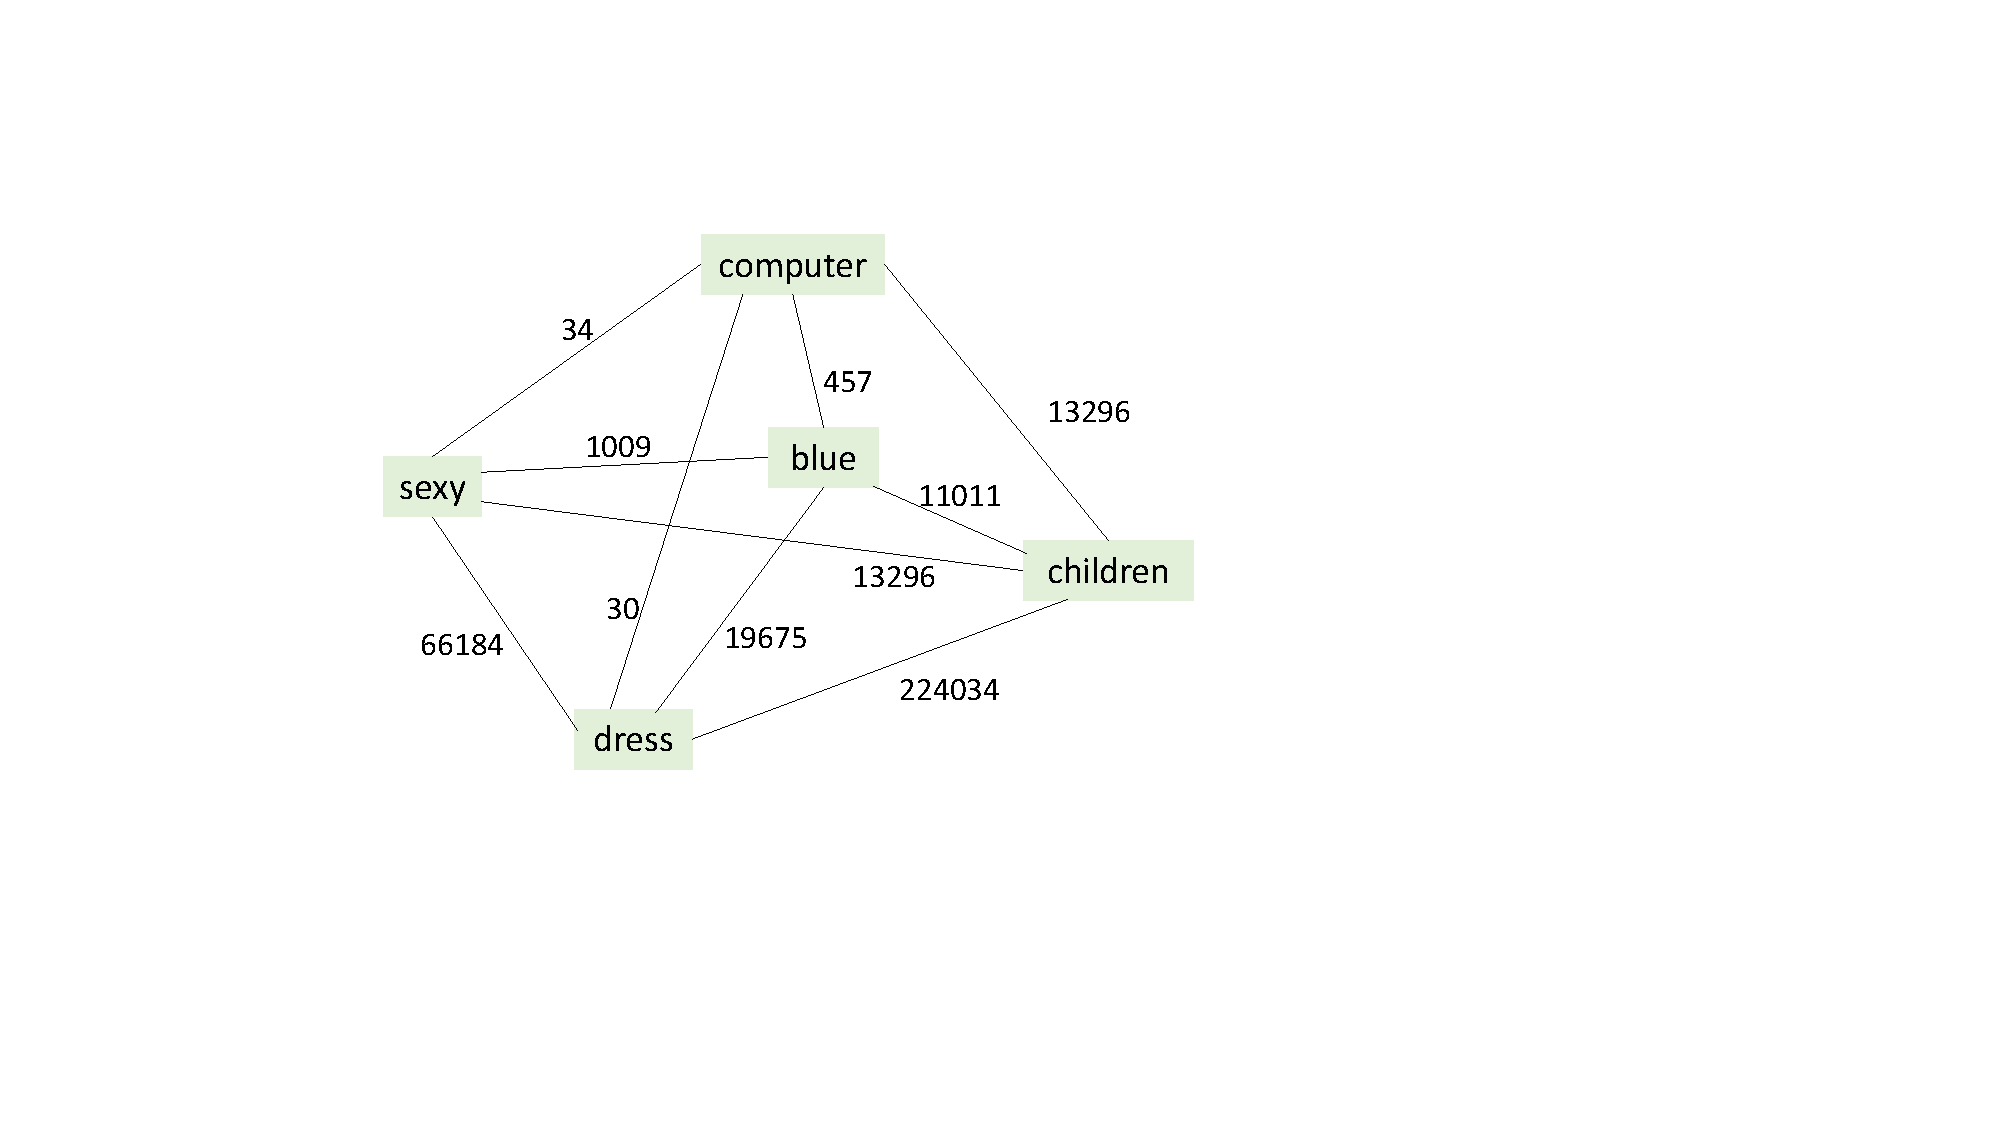
\includegraphics[width=0.8\columnwidth]{images/associationNetColor.pdf}
	\caption{A fragment of our constructed net}
	\label{fig:net}
\end{figure}

The distribution of users on the e-commerce platform is not uniform. For example, number of female users are much more than male users. This leads to the phenomenon that occurrence of word pair (electric, dress) may larger than (electric, torch) even though (electric, dress) is more unreasonable. The reason is that there are lots of female users search for \textit{dress} so even the strange combination of words may still appear much more times than a normal collocation with \textit{torch}. 
 
Mutual information is a suitable criterion to measure the dependency of two words. If word A appears $x$ times in the query corpus, word B appears $y$ times, the word pair (A,B) appears $z$ times, and the total number of words is $N$, then the mutual information between word A and B is defined as:
\begin{equation}
I(A,B) = log\frac{P_r(A\wedge B)}{P_r(A)\times P_r(B)}
\end{equation}
and can be estimated as:%using:
\begin{equation}
I(A,B) \approx log\frac{z\times N}{(x+z)\times (y+z)}
\end{equation}

We use mutual information to calculate the strength of word associations in our constructed net, which noted as ``plausibility".
%will be regarded as reasonability of this word pair.
%\KZ{Instead of reasonability, use the word ``plausibility''.}
For a phrase $T=(w_1, ..., w_m)$, there may not only two words, we need to calculate the overall plausibility $R$ as:
\begin{equation}
P(T) = \frac{2}{m*(m-1)}\sum_{i=1}^{m-1}\sum_{j=i+1}^{m}I(w_i, w_j)
\end{equation}

%Besides, as our positive sample should be clear, coherent and common, but a query may contain lots of noise,
%Besides, as there are countless combination of words, for example, the combination of \textit{color} and most daily things are reasonable, but the user query in 7 days may not cover all. Hence, we make another assumption after observing the result: Pair never appear $\neq$ unreasonable, BUT rare appear $=$ unreasonable. This assumption is a little strong but efficient for us to constrain the scope of positive samples.

%Hence we do not take the 2-word query into account \mx{should extend to 3 or more words phrase} if any word in the query or the word pair haven't appeared in our net.   

Besides, as most positive samples are common enough, we remove the phrase which contains any rare word that appears less than 100,000 in our graph. If all word pairs in a phrase doesn't exist in our graph, this phrase will also be filtered. Then, the remained samples are ranked according to their overall plausibility score from small to large to get the most unreasonable phrase list.

To evaluate the effectiveness of the above method, we test on our 10,000 preliminary annotated phrases. %as example.
After removing rare word, 6381 phrases (include 94 positive samples) are removed where the rate of positive phrase is 1.47\%. After removing non-exist word pair, another 107 samples (include 9 positive phrases) are removed. Finally, 3512 phrases (include 167 positive phrases) remain. Among previous 15\% of these samples, 77 positive ones among total 526 samples are found, where the rate of positive samples achieves 15.4\%, remarkably improves compared to 2.92\% on the 10,000 randomly selected on preprocessed raw data.
%showing the validity of the constructed graph.

%Therefore, we apply 
Seeing the validity of the constructed graph, the above method is applied on our whole unlabeled preprocessed 4,081,254 raw data, 1,176,922 are kept. After rank of overall plausibility score, %we fetch the previous 15\% (equals to 176,538 samples) for further human annotation.
we fetch the previous\JQ{front} 18,000 samples for further human annotation due to the limited resources.

%\subsection{Phrase annotation \& rewriting}
%When annotate and rewriting samples, annotator are both given a guideline to follow.

\textit{Step2: Phrase Annotation}

This part describes the guideline that the annotators are given to follow.
%During this period, annotators need to judge if a phrase is a commonsense contradiction. 
For given short phrases, annotators need to first filter the low-quality samples, then judge if it is an appropriate commonsense contradiction sample.\JQ{此句对吗}
\begin{enumerate}
	\item Phrase belongs to any one of these four cases can be directly ignored\JQ{deleted}: 
	%satisfies 
	\begin{itemize}
		\item [-] Reasonable phrase. %Correct commonsense phrase.
		\item [-] Not clear and can not distinguish the subject in a phrase, such as "children deer''(儿童麋鹿).\JQ{这条没懂}
		\item [-] Contain ambiguous subject, such as "cat" in "silk cat''(桑蚕丝猫咪), referring to an animal or an ornament.
		\item [-] Contain word that is too rare (i.e. unfamiliar to the annotator)
	\end{itemize}
	\item Judge the phrase to be unreasonable if it belongs to the four following commonsense contradiction category:
	\begin{itemize}
		\item [-] Several modifiers for one subject and commonsense contradiction exists between modifiers. For example, in ``Europe Korean curtain''(欧韩窗帘), two national modifiers are contradictory.
		\item [-] The modifier is contradictory with the intrinsic property of subject itself. For example, ``vitreous porcelain''(玻璃青花瓷), ``thermal ice bag''(保温冰袋), ``children sexy dress''(儿童性感连衣裙), ``boy night skirt''(男童睡裙).
		\item [-] The modifier is strange for describing the subject %'s intrinsic property 
		according to common sense, such as ``Walking alarm clock''(会走的闹钟), ``vacuum keyboard''(真空键盘).
	\end{itemize}
\end{enumerate}

%\KZ{You need to say how many human annotators are employed; what is the inter-judge
%agreement (assuming each entry is annotated by multiple judges.}
%Due to the resource limit, we only use the previous 18,000 of fetched data and distribute them to 6 person.  
We distribute these 18,000 fetched data to 6 person who is asked to choose intuitively the unreasonable phrase by their common sense. Finally, 15,567 commonsense contradiction samples are returned, hitting the rate of \textbf{86.48\%}, which is much larger than the original rate of \textbf{2.92\%}.

\textit{Step3: Negative Samples Generation}

Because human rewriting is costly, we consider a more efficient way to obtain the associated negative sample 
%(reasonable one) 
for each collected commonsense contradiction sample. The plausibility score $P$ is reused in this part: for each positive sample,
%(commonsense contradiction one)
we pair it with a short phrase in our total preprocessed query data that satisfies the following rules:
\begin{itemize}
	\item Describe the same object.
	\item Possess the same number of characters.
	\item Only one word in the original positive sample is replaced. %Only one word different from the original positive sample according to the result of segmentation.
	\item Plausibility score is higher than the original sample.
\end{itemize}

This automatic generation helps us to get 12,416 pairs of short phrases.

%\subsection{Additional Verification}
\subsection{Dataset Validation}
For further improving the quality of dataset, we ask different crowd workers to judge which phrase is more reasonable or can not distinguish between two phrases. We also set 300 checking problems. The annotated pairs from annotators who choose correctly on more than 80\% checking problems will be counted into the final collection. Figure \ref{fig:crowd} is the crowdsourcing web interface of data verification.\JQ{right?}

\begin{figure}
	\centering
	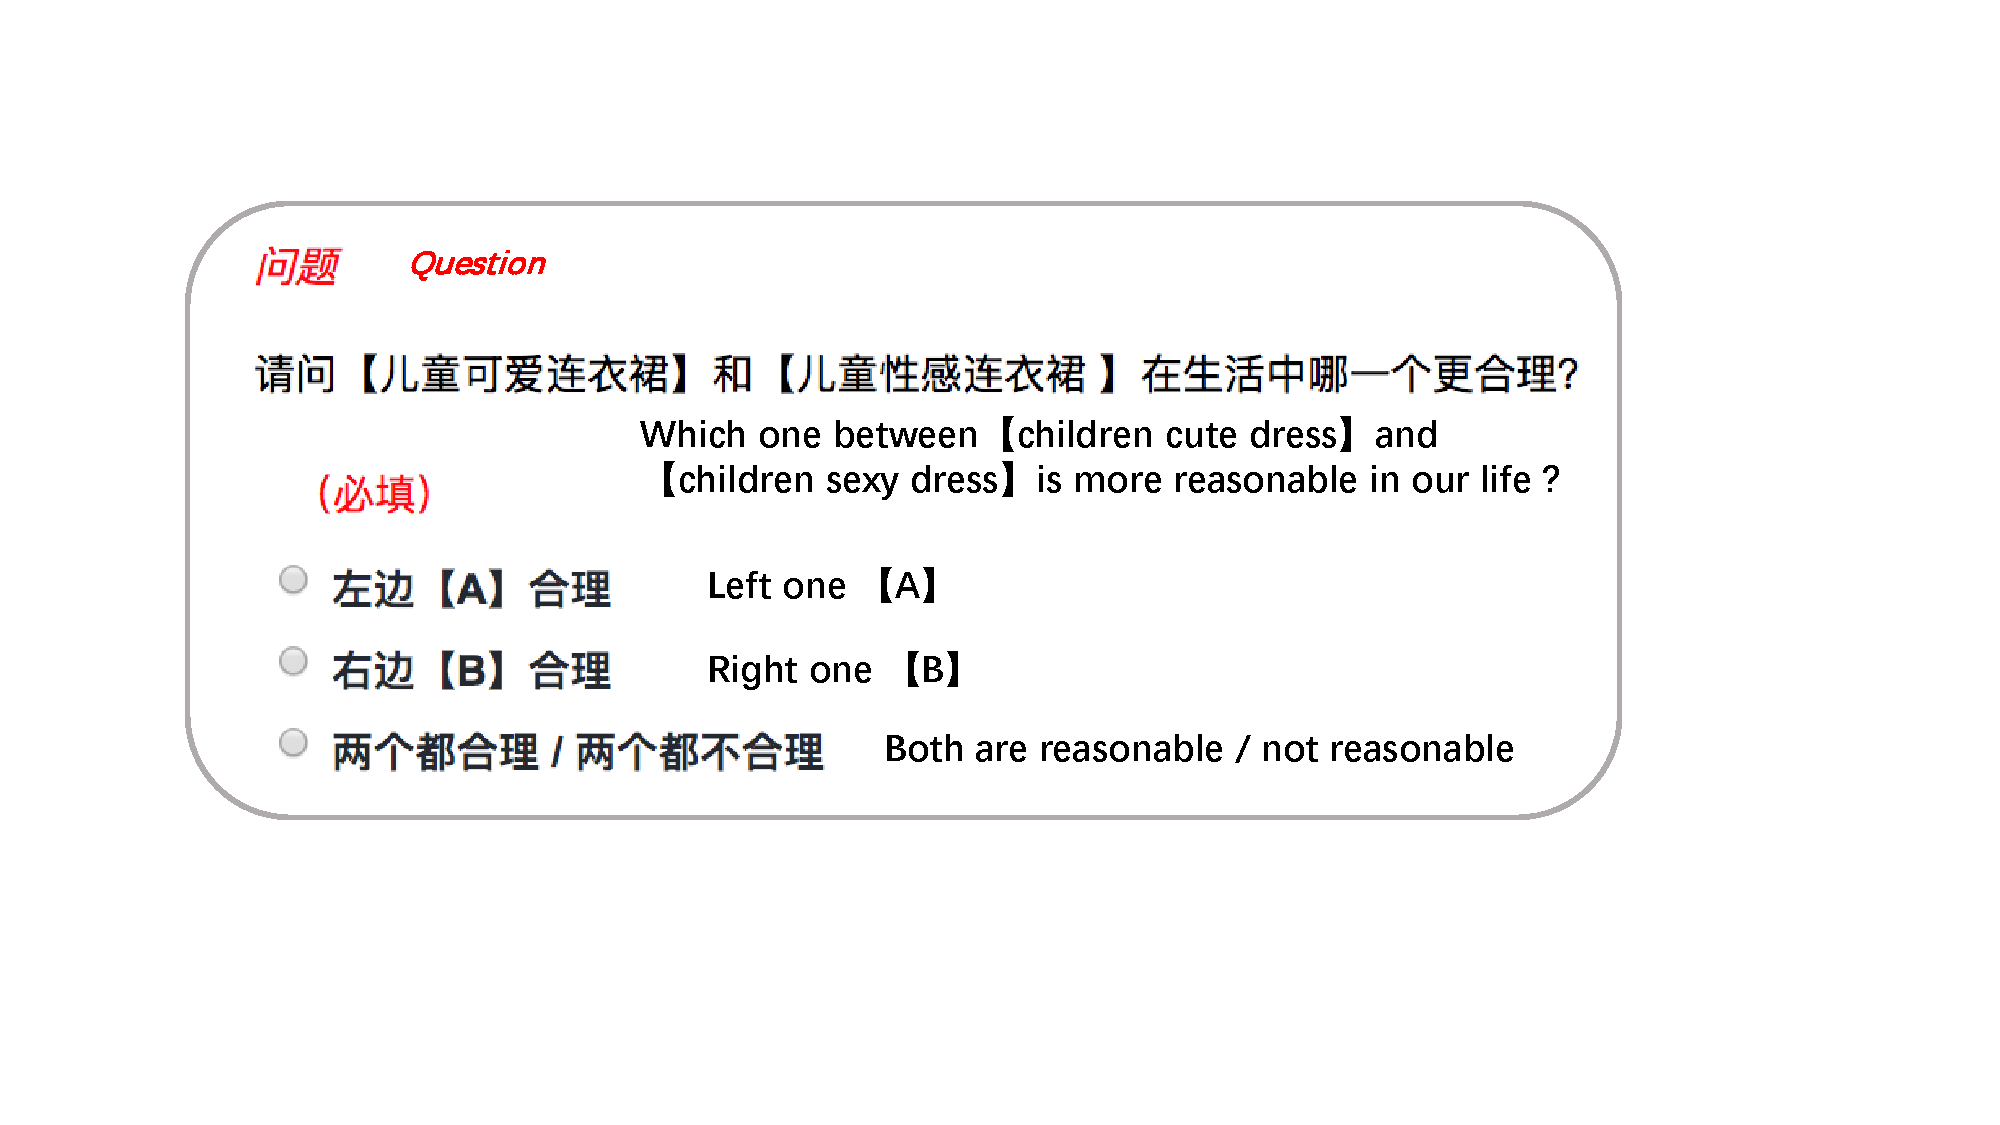
\includegraphics[width=0.95\columnwidth]{images/crowdPage.pdf}
	\caption{The crowd-facing web interface used to filter the dataset}
	\label{fig:crowd}
\end{figure}

Each sample is judged by 5 person, and we only keep those pairs that gain more than 4 same votes. After this step, we finally obtain our \textbf{CoCo} (\textbf{Co}mmonsense \textbf{Co}ntradiction) dataset, which contain 9,229 short phrase pairs \footnote{CoCo dataset can be found at \url{http://release_after_acception}}.


%\subsubsection{Phrase rewriting} After obtaining those commonsense contradiction samples, annotators are asked to rewrite them their relative negative ones which satisfy commonsense. For example, "sexy children dress" can be rewritten as "cute children dress". However, there are numerous rewrite ways. A rewrite is admitted if it accord with the following principles:
%\begin{enumerate}
%	\item Only one word is modified.
%	\item Do not modify the subject as subject is the core of phrase.
%	\item Property (include part of speech and type) of modified word should be the same with the original word. For example, verb should be changed to verb, same to noun, adjective and etc. The modified word should be similar with the original one in some aspect, which could confuse those pretrained model like BERT.
%	\item The replaced word should keep same length with the original word. Because we don't want length of word itself influence the judgement of model, either thick or dilute the weight of subject.
%	\item Try to avoid universal modifier in rewriting word, such as "personalized", "popular", color or nation. Because those universal modifiers hardly reveal any useful information for judgement. For example, human can not judge which is more reasonable between "personalized dress" and "popular dress" according to their commonsense knowledge.
%\end{enumerate} 
